\subsection{Hierarchical clustering}\label{sec:hc}
Hierarchical clustering is a general family of clustering algorithms that builds nested clusters by merging or splitting them successively. This hierarchy of clusters can be represented as a tree (or dendrogram). The root of the tree is the unique cluster that gathers all the samples, the leaves being the clusters with only one sample. To perform hierarchical clustering the AgglomerativeClustering function from scikit-learn was used. Note that this approach was applied just to samples, nothing was done to classify genes. In this case genes are only dimensions in which samples are represented.

The AgglomerativeClustering object performs a hierarchical clustering using a bottom up approach: each observation starts in its cluster, and clusters are successively merged. The linkage criterium determines the metric used for the merging strategy. 
First of all, distances between all elements are estimated; in this work was used standard euclidean distance. Then elements are merged using a linkage criterion; in this work standard Ward linkage was used. The Ward linkage minimizes the sum of squared differences between the distances. It is actually a variance-minimizing approach. Here the specific setting used in this work.
\begin{lstlisting}[style=mypython]
from sklearn.cluster import AgglomerativeClustering
AgglomerativeClustering(
    affinity='euclidean',
    compute_full_tree='auto',
    linkage='ward',
    n_clusters=x,
    )
\end{lstlisting}
In figure~\ref{fig:topic/hc} an example of a hierarchical clustering. Note that nodes with short distance are linked firstly.
\begin{figure}[htb!]
	\centering
	\begin{minipage}{0.35\textwidth}
		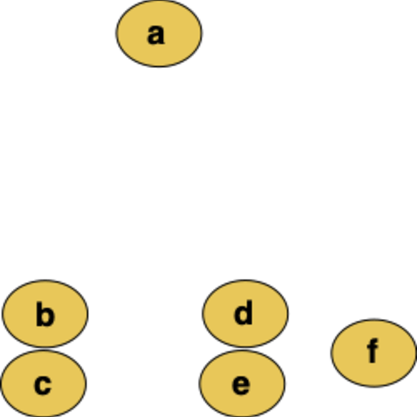
\includegraphics[width=0.8\linewidth]{pictures/topic/clusters.pdf}
	\end{minipage}
\hspace{3mm}
	\begin{minipage}{0.35\textwidth}
			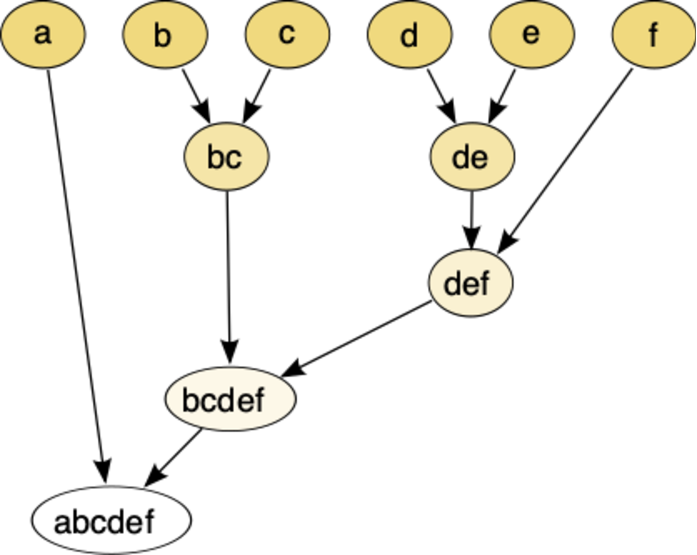
\includegraphics[width=0.9\linewidth]{pictures/topic/hierarchical_clustering_simple_diagram.pdf}
	\end{minipage}
\caption{Example of hierarchical clustering}
\label{fig:topic/hc}
\end{figure}

\subsection{LDA}\label{sec:lda}
Latent Dirichlet Allocation is another approach to topic models. It has got more restrictive priors and needs some parameters to be set. It uses some different methods to maximize the posterior probability to observe some latent variables given the data.
As well described in~\cite{Zhou2016} LDA is a generative model and can be summarised as follows:
\begin{itemize}
	\item for each topic k generate $\beta_k\sim \text{Dirichlet}(\bullet |\eta)$
	\item for each document $d$ generate $\theta_d\sim \text{Dirichlet}(\bullet|\alpha)$
	\item for each word in $d$ 
	\begin{itemize}
		\item generate $z\sim \text{Multinomial}(\bullet|\theta_d)$
		\item generate $w\sim \text{Multinomial}(\bullet|\beta)$
	\end{itemize}
\end{itemize}
\begin{figure}[htb!]
	\centering
	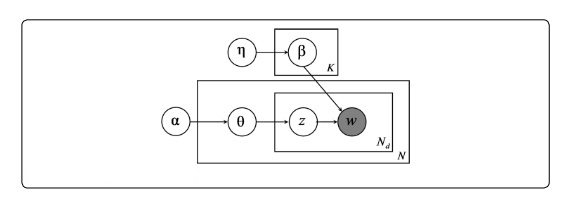
\includegraphics[width=0.65\linewidth]{pictures/topic/LDA.jpeg}
	\caption{LAD scheme}
	\label{fig:LDA}
\end{figure}
this process is summarized in figure~\ref{fig:LDA}. These steps are useful to maximize the posterior probability
\begin{equation}\label{eq:lda}
P(w, z,\beta, \theta| \alpha, \eta)=\prod_{d=1}^N P(\theta_d | \alpha)\prod_{n=1}^{N_d} P(w_{dn}|z_{dn},\beta)P(z_{dn}|\theta_d)\prod_{k=1}^KP(\beta_k|\eta)
\end{equation}
where
\begin{itemize}
	\item $N$ is the number of documents
	\item $K$ is the number of topics as set by the user
	\item $w$ are words
	\item $N_d$ is the number of words in document d
	\item $\alpha$ and $\eta$ are parameters of the model (usually $\eta=0.01$ and $\alpha=50/K$)
	\item $P(\theta | \alpha)$ and $P(\beta|\eta)$ are Dirichlet distributions
\end{itemize}
When $\beta$, $\theta$ and $z$ are estimated, the outputs are the topic distribution in documents $P(z|d)$ and the word distribution in topics $P(w|z)$.